\documentclass[12pt]{article}
\usepackage[T1]{fontenc}
\usepackage[french]{babel}
\usepackage{hyperref}
\usepackage{float}
\usepackage{graphicx}
\usepackage{caption}
\usepackage{listings}
\usepackage[dvipsnames]{xcolor}

\lstset{
    language=Java,
    numbers=left,
    frame=single,
    commentstyle=\color{Green},
    keywordstyle=\color{blue},
    stringstyle=\color{red},
    numberstyle=\tiny,
    breaklines=true
}

\captionsetup[figure]{labelformat=empty}

\begin{document}
    \title{Rapport Projet 2024}
    \author{Romain MOALIC \and Thomas DOGUET}
    \maketitle
    \newpage
    \tableofcontents
    \newpage

    \section{Page d'Accueil}
        Bienvenue sur la page d'accueil de ce document. Ce document est le rapport pour le projet de fin de semestre "fil rouge" dans la matière "Aide à la décision et intelligence artificielle".
		\begin{figure}[H]
			\centering
			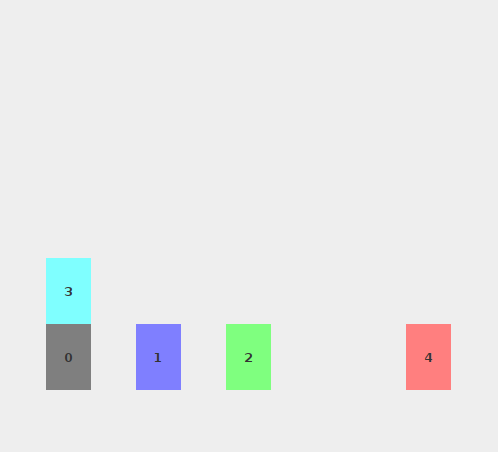
\includegraphics[width=1\textwidth]{image/accueil.png}
		\end{figure}
    \newpage % Nouvelle page

    % Page avec trois éléments
    \section{Mise en place primaire}
        Nous avions pour consigne de mettre en place un monde de blocs avec tout d'abord une mise en place de base, divisée en quatre sections.
        
        \subsection{Modélisation Attribut-Valeur}
            Cette partie du TP nous a permis de mettre en place les "bases" :
            \begin{itemize}
                \item Nous avons créé les variables, c'est-à-dire chaque élément de notre monde de blocs :
                    \begin{itemize}
                        \item Elles sont composées d'un nom et d'un domaine.
                        \item Les méthodes créées sont des méthodes d’accession au domaine ou au nom, et une autre méthode "equals" permet de vérifier si deux variables sont les mêmes.
                    \end{itemize}
                \item Nous avons créé les variables booléennes, un type de variable dont le domaine est un ensemble contenant les deux booléens.
                \item Nous avons créé les contraintes, divisées en plusieurs types :
                    \begin{itemize}
                        \item Les contraintes de différences, elles prennent en compte deux variables et vérifient grâce à la méthode "IsSatisfied" si elles sont bien différentes.
                        \item Les contraintes unaires, elles prennent en compte une variable et un sous-ensemble de leur domaine, et vérifient grâce à la méthode "IsSatisfied" si la variable existe.
                        \item Les contraintes d'implication, elles prennent en compte deux variables (\texttt{v1} et \texttt{v2}) et deux sous-ensembles de leurs domaines (\texttt{s1} et \texttt{s2}) :
                            \begin{itemize}
                                \item Elles sont satisfaites si ce n’est pas une valeur de \texttt{s1} qui est affectée à \texttt{v1}, quelle que soit la valeur affectée à \texttt{v2}.
                            \end{itemize}
                    \end{itemize}
            \end{itemize}

        \subsection{Planification}
            Cette partie du TP consistait à résoudre des problèmes, c'est-à-dire partir d'un état initial pour arriver à un état final. Pour cela :
            \begin{itemize}
                \item Nous avons d’abord créé les actions :
                    \begin{itemize}
                        \item Une action a une précondition (liste de variables nécessaires) et une liste d’effets (état souhaité).
                        \item Une action vérifie si elle est applicable, c'est-à-dire si ses préconditions sont respectées dans l'état actuel.
                    \end{itemize}
                \item Nous avons créé les buts, qui servent à vérifier que les préconditions pour appliquer une action sont bien respectées.
                \item Nous avons ensuite créé une série de \texttt{Planners} pour résoudre les problèmes selon différents algorithmes :
                    \begin{itemize}
                        \item Le parcours en largeur (\texttt{BFS}).
                        \item Le parcours en profondeur (\texttt{DFS}).
                        \item Le parcours suivant l'algorithme de Dijkstra.
                        \item Le parcours suivant l'algorithme \texttt{A-star}.
                    \end{itemize}
                    Chaque classe contient une méthode \texttt{plan}, qui retourne une liste d’actions à effectuer pour résoudre le problème. Elles sont équipées de compteurs pour mesurer leur efficacité en différents cas.
                \item Enfin, nous avons créé une interface heuristique pour estimer des quantités comme un nombre d’actions ou des blocs avec une propriété particulière.
            \end{itemize}

        \subsection{Problème de satisfaction des contraintes}
            Ici, nous nous sommes intéressés à transformer un état invalide en un état respectant toutes les contraintes :
            \begin{itemize}
                \item Nous avons créé un \texttt{Solver} :
                    \begin{itemize}
                        \item Un solver transforme un état invalide en un état valide en suivant différents algorithmes :
                            \begin{itemize}
                                \item L'algorithme de \texttt{Backtracking}.
                                \item L'algorithme \texttt{MAC}.
                            \end{itemize}
                        \item Chaque solver a une méthode \texttt{solve} qui retourne un état "résolu".
                    \end{itemize}
                \item Nous avons ensuite créé une classe \texttt{ArcConsistency} :
                    \begin{itemize}
                        \item \texttt{enforceNodeConsistency} : Supprime les valeurs non valides dans les domaines des variables. Retourne \texttt{false} si une contrainte n’est pas satisfaite.
                        \item \texttt{revise} : Supprime les valeurs impossibles pour une variable, en fonction des contraintes avec d'autres variables.
                        \item \texttt{ac1} : Applique l'algorithme AC1 pour filtrer les domaines.
                    \end{itemize}
                \item Enfin, nous avons créé deux interfaces d’heuristiques :
                    \begin{itemize}
                        \item \texttt{Heuristiques de Variable}.
                        \item \texttt{Heuristiques de Valeur}.
                    \end{itemize}
                    Ces heuristiques ont été étendues dans des classes concrètes :
                    \begin{itemize}
                        \item \texttt{RandomValueHeuristic} : Mélange la liste de valeurs de façon aléatoire.
                        \item \texttt{NbConstraintsVariableHeuristic} : Classe les variables en fonction de leur occurrence dans les contraintes.
                    \end{itemize}
            \end{itemize}

        \subsection{Extraction des connaissances}
                	Nous avons maintenant mis en place l'extraction des connaissance en plusieurs étapes

    	\begin{itemize}

    		\item la mise en place de la classe itemset, qui représente un ensemble d'items (Variables booléennes et leurs fréquence.

    		\item la mise en place de la classe AssociationRule, qui représente une règle d'association, qui est composé d'ensembles d'items, une prémisse et une conclusion, une fréquence et une confiance

    		\item Maintenant notre objectif était de d'extraire ces règles et ensembles d'items, grâce à des miners, les miners sont équipés d'une méthode extract, qui renvoient des ensembles d'ensemble d'items ou de règles d'association, en fonction de condition (les fréquences et confiances minimales pour les règles d'association et les fréquences minimales pour les ensembles d'items)

    		Nous avons par exemple implémenté un miner d'items set en fonction de l'algorithme Apriori, ou bien un miner de règle d'association de manière brute(BruteForce)

    		\item Nous avons pour finir créer la représentation d'une base de donnée de d'itemset, qui contient les itemset "actuels" et la liste de transactions effectuées auparavant.
            
		\end{itemize}
    \section{Mise en place concrète du Monde de Bloc}
        Afin de mettre en place un monde de blocs, nous avons réutilisé toutes les étapes précédentes de la mise en place :
            \subsection{Attribut-Valeurs}
                \begin{itemize}
                    \item Nous avons créé les variables des blocs (\texttt{on}, \texttt{fixed}, \texttt{free}) en suivant une logique systématique.
            \subsection{Contraintes}
                \begin{itemize}
                    \item Chaque couple de blocs différents ne peut pas occuper la même position.
                    \item Si un bloc est supporté par un autre, celui-ci devient fixe.
                    \item Si une pile contient un bloc, elle n’est pas libre.
                \end{itemize}
           \subsection{Contraintes de Régularité}
                \begin{itemize}
                    \item Les écarts entre blocs dans une pile doivent être réguliers.
                \end{itemize}
            \subsection{Contraintes de Croissance}
                \begin{itemize}
                    \item Chaque bloc supérieur a une valeur plus grande que celui situé en dessous.
                \end{itemize}
            
            \subsection{Planification} : Nous avons mi en place la planification afin de résoudre notre monde de block, pour cela
    \begin{itemize}
        \item Nous avons défini les différentes actions possibles dans ce monde. Il existe quatre types d'actions :
        \begin{itemize}
            \item 1. Déplacer un bloc \(b\) du dessus d’un bloc \(b'\) vers le dessus d’un bloc \(b''\),
            \item 2. Déplacer un bloc \(b\) du dessus d’un bloc \(b'\) vers une pile vide \(p\),
            \item 3. Déplacer un bloc \(b\) du dessous d’une pile \(p\) vers le dessus d’un bloc \(b'\),
            \item 4. Déplacer un bloc \(b\) du dessous d’une pile \(p\) vers une pile vide \(p'\).
        \end{itemize}
        Pour cela, nous avons mis en place la classe \texttt{BWAction}, qui parcourt les différents blocs ou piles et génère toutes les actions possibles.
        
        \item Nous avons également implémenté trois heuristiques, qui servent à fournir des informations ou à évaluer l'efficacité de notre planification :
        \begin{itemize}
            \item 1. Une heuristique comptant le nombre de blocs mal placés,
            \item 2. Une heuristique comptant le nombre de blocs bloqués sous un autre,
            \item 3. Une heuristique calculant l’union des blocs bloqués et mal placés.
        \end{itemize}
    \end{itemize}
    
\subsection{Problème de satisfaction des contraintes}  
Nous n’avons pas eu besoin de créer de représentation spécifique pour cette partie. Nous avons simplement créé des exemples montrant que nos solveurs implémentés précédemment suffisent.

\subsection{Extraction de connaissances}  
Pour représenter l'extraction de connaissances, nous avons tout d'abord créé d’autres types de variables :
\begin{itemize}
    \item 1. \texttt{On\_b\_b'} : Pour chaque couple de blocs différents \(\{b, b'\}\), une variable prenant la valeur \texttt{true} lorsque le bloc \(b\) est directement sur le bloc \(b'\) (et \texttt{false} sinon).
    \item 2. \texttt{Ontable\_b\_p} : Pour chaque bloc \(b\) et chaque pile \(p\), une variable prenant la valeur \texttt{true} lorsque le bloc \(b\) est sur la table dans la pile \(p\) (et \texttt{false} sinon).
\end{itemize}
Nous avons créé une classe \texttt{BWDatamining} qui récupère les différentes variables, en génère de nouvelles et construit une base de données grâce aux bibliothèques fournies.

\subsection{Vue}  
Pour créer la vue, nous avons développé une classe \texttt{Vue} qui utilise le code et les bibliothèques données dans l'énoncé. Ce code est divisé en trois méthodes :
\begin{itemize}
    \item Une méthode permettant de créer un monde de blocs à partir de l’état donné en paramètre,
    \item Une méthode pour afficher un état,
    \item Une méthode pour afficher le déroulé d’un plan de résolution.
\end{itemize}

\subsection{Mise en place de la vue}  
Pour intégrer la vue, nous avons utilisé la classe \texttt{Thread}. En utilisant ses méthodes, il suffit de créer un thread et d’appeler sa méthode \texttt{run()} pour lancer l’affichage.

        	
        \end{itemize}
        \newpage
	\section{Explication des executables}
		La commande pour tous compiler est la suivante : javac -cp "lib/*" -d build src/**/*.java src/**/**/*.java
		
		\subsection{Executable des contraintes}
			La commande pour lancer l'executable des tests des contraintes est : java -cp build blockWorld.modelling.BWmodellingExecutable .
			Cette classe permet des tester les contraintes basiques, regulières, croissante ansi que regulière et croissante en même temps. Pour vérifier chaque contraintes, on définit un état qui seras lui à vérifier :
			\lstinputlisting[title=BWmodellingExecutable.java, firstline=18, lastline=23]{../src/blockworld/modelling/BWmodellingExecutable.java}
			Cette matrice est converti en une map qui représente l'état de cette matrice pour ensuite parcourir chaque élement de cette état pour vérifier les contraintes :
			 \lstinputlisting[title=BWmodellingExecutable.java, firstline=54, lastline=58]{../src/blockworld/modelling/BWmodellingExecutable.java}
			 Un affichage est ensuite fait si toutes les contraintes sont satisfaites\\
			 Les images montrent le test pour les contraintes basiques, les mêmes test sont effectués pour les contraintes régulières, croissante et régulières + croissante.\\Voici le résultat ! :\\
			 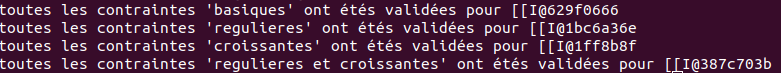
\includegraphics[width=1\textwidth]{image/resContraintes.png}
			 
		\subsection{Executable des Planner}
			La commande pour lancer l'executable des tests des planner est : java -cp build:lib/blocksworld.jar blockWorld.planning.BWplanningExecutable .\\\\
			Cette classe permet de tester les planner avec le dfs, bfs, astar et c'est différentes heuristiques et dijkstra. Pour ça on définit un état de base et un autre état qui vaut au but a atteindre.
			\lstinputlisting[title=BWplanningExecutable.java, firstline=30, lastline=42]{../src/blockworld/planning/BWplanningExecutable.java}
			En utlisant le dfs et autres, on peut récuperer le plan nécessaire avec une liste d'actions, le temp d'execution du planner utilisé et le nombre de noeuds visité pour obtenir le résultat.
			\lstinputlisting[title=BWplanningExecutable.java, firstline=49, lastline=55]{../src/blockworld/planning/BWplanningExecutable.java}
			Un affichage est ensuite fait, montrant le temps d'execution, le nombre de noeuds visité et la taille du plan d'actions trouvé .\\
			Les mêmes test sont faient pour le dfs, bfs, astar avec les différents heuristiques ([1], [2], [1,2]) et de même pour djikstra.\\
			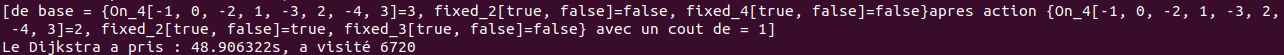
\includegraphics[width=1\textwidth]{image/resPlanning.png}
			
		\subsection{Executables des Solvers}
			Les commandes pour lancer les executables des tests des solvers sont :
			\begin{itemize}
				\item java -cp build:lib/blocksworld.jar \\blockWorld.planning.BWRegularityConstraintsExecutable
				\item java -cp build:lib/blocksworld.jar \\blockWorld.planning.BWIncreasingConstraintsExecutable
				\item java -cp build:lib/blocksworld.jar \\ blockWorld.planning.BWRegularityAndIncreasingConstraintsExecutable
			\end{itemize}
			Ces classes permettent de tester les solvers pour les différentes contraintes, donc regulières, croissante et les deux en mêmes temps. Pour ça on recuperes les différentes contraintes pour les appliquer.
			\lstinputlisting[title=BWRegularityAndIncreasingConstraintsExecutable.java, firstline=32, lastline=36]{../src/blockworld/planning/BWRegularityAndIncreasingConstraintsExecutable.java}
			En utilisant nos différents solvers : backtrack, mac et macHeuristique on a réussie à recuperer les résultat de nos solvers ainsi que le temps d'éxecution: 
			 \newpage
			\lstinputlisting[title=BWRegularityAndIncreasingConstraintsExecutable.java, firstline=39, lastline=43]{../src/blockworld/planning/BWRegularityAndIncreasingConstraintsExecutable.java}
			Voici le résultat :\\\\
			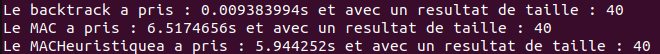
\includegraphics[width=1\textwidth]{image/resSolver.png}
			Le resultat du macHeuristique n'est pas bon et nous n'avons pas réussi à trouver la raison malheureusement\\
			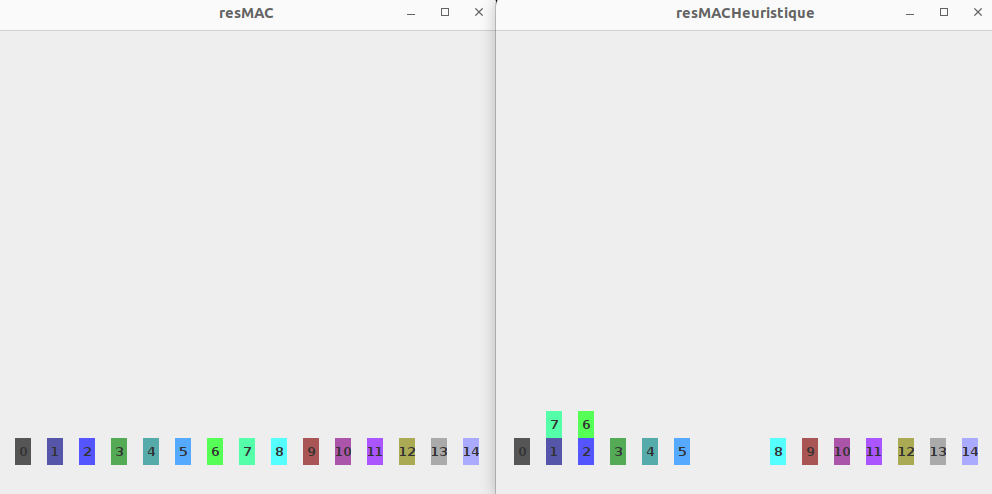
\includegraphics[width=1\textwidth]{image/erreur.png}
		
		\subsection{Executable datamining}
			La commande pour lancer l'executable datamining est : java -cp build:lib/bwgenerator.jar blockWorld.datamining.BWDataminingExecutable
			\\Cette classe permet d'afficher les fréquences chercher des différentes variables (blocs et piles) :\\
			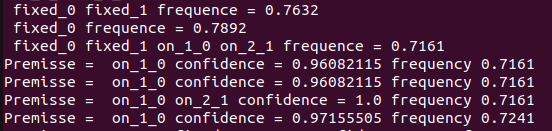
\includegraphics[width=1\textwidth]{image/frequence.png}
\end{document}
